\section{Qualidade de Software}

\subsection{Medição e Análise}

GQM é uma abordagem \textit{top-down} orientado a metas para a mensuração de produtos e processos de software, ou seja, é um processo para definição e interpretação de métricas de software. \cite{junior}

A ideia base desta abordagem é, para cada meta estabelecida dentro da organização identificar questões possíveis de serem respondidas com a análise de medidas coletadas para métricas, sendo a medição então fundamentada em metas que a organização visa alcançar.

O modelo GQM é composto por três níveis de acordo com a figura \ref{fig:gqm} \cite{junior}:

\begin{figure}[h!]
	\centering
  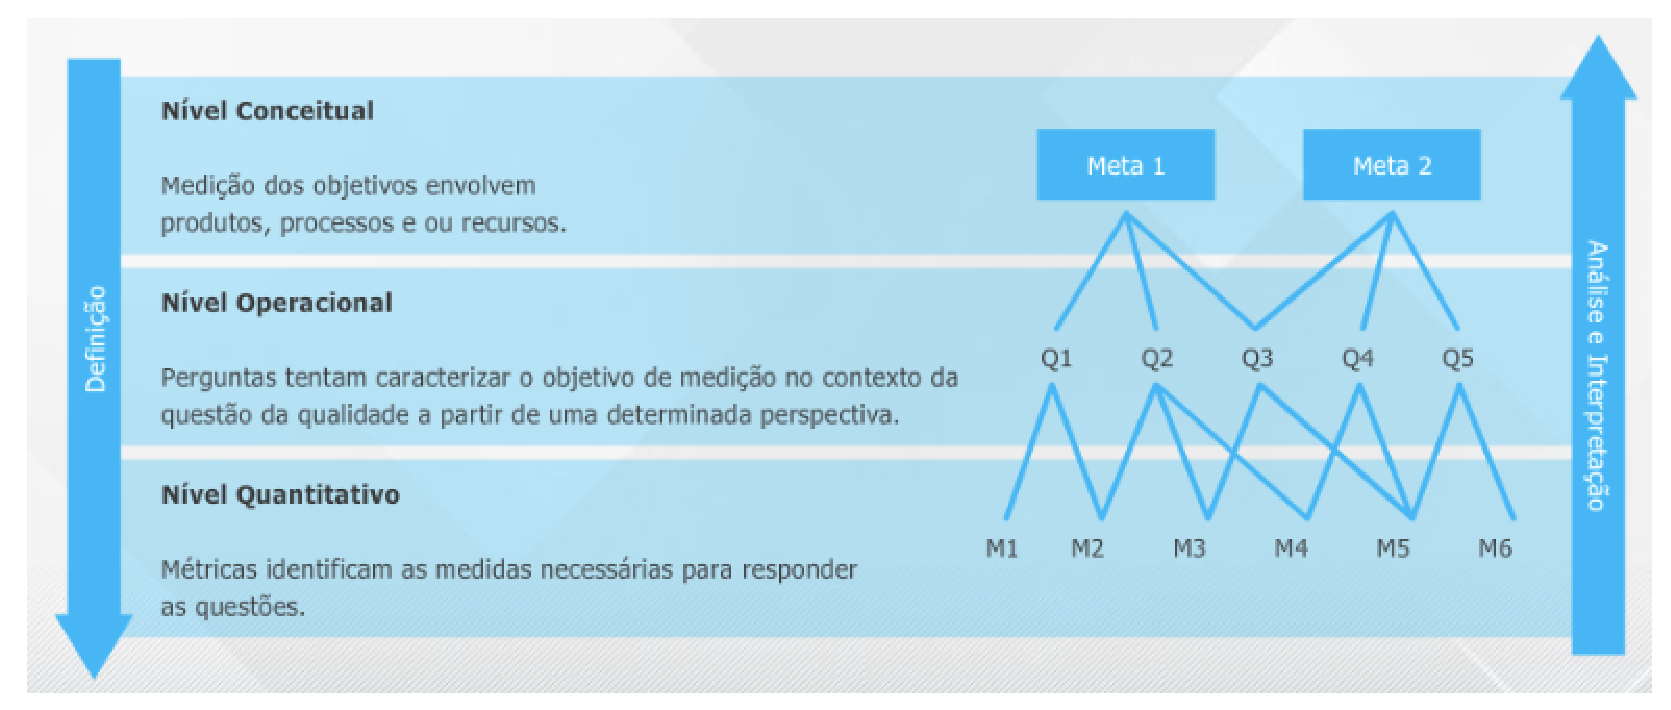
\includegraphics[keepaspectratio=true,scale=0.5]{figuras/gqm.eps}
  \caption[Níveis do GQM.]{Níveis do GQM. Fonte: \cite{junior}}
	\label{fig:gqm}
\end{figure}

\begin{itemize}
  \item \textbf{Conceitual}: Uma meta é definida para um objetivo, envolvendo produtos, processos ou recursos.
  \item \textbf{Operacional}: Um conjunto de perguntas é elaborado com relação a cada objetivo identificado.
  \item \textbf{Quantitativo}: Um conjunto de métricas é estabelecido, de maneira a atender a cada pergunta elaborada.
\end{itemize}

Um processo de medição de software direcionado aos objetivos produz medidas que provêem informações para importantes
questões de negócio, previamente identificadas. Uma vez que as medidas podem ser rastreadas de volta aos objetivos da
organização \cite{junior}.

\subsection{Verificação e Validação}

propósito do processo de verificação é confirmar que cada serviço e/ou produto de trabalho do processo ou do projeto atende apropriadamente os requisitos especificados \cite{pressman1}

O processo de verificação é detalhado pelo guia, segundo o \cite{softex}, em 6 tarefas gerais:

\begin{itemize}
  \item \textbf{VER 1}: Identificar os produtos de trabalho a serem verificados.
  \item \textbf{VER 2}: Desenvolver e implementar uma estratégia de verificação, com definição de um cronograma,
    revisores envolvidos, métodos para verificação e qualquer material a ser utilizado na verificação.
  \item \textbf{VER 3}: Identificar critérios e procedimentos para verificação dos produtos de trabalho,
    além da definição do ambiente de verificação.
  \item \textbf{VER 4}: Executar revisão por pares e testes e atividades de verificação.
  \item \textbf{VER 5}: Identificar e registrar defeitos.
  \item \textbf{VER 6}: Analisar os resultados gerados e encaminhar aos envolvidos.
\end{itemize}

O objetivo da validação é validar que um produto de software atenderá a seu objetivo quando colocado no ambiente para o
qual foi desenvolvido \cite{sommerville}.

De forma geral o processo de validação tem seu foco em como avaliar a qualidade de um produto ou componente de produto,
assegurando que os objetivos e ou necessidades dos clientes sejam atendidas quando colocado em seu ambiente de produção,
ou seja, o objetivo da validação é garantir que o produto correto está sendo desenvolvido \cite{softex}.

O processo de validação é detalhado pelo guia, segundo o \cite{softex}, em 7 tarefas gerais, como resultados esperados:

\begin{itemize}
  \item \textbf{VAL 1}: Identificar os produtos de trabalho a serem validados.
  \item \textbf{VAL 2}: Desenvolver e implementar uma estratégia de validação, com definição de um cronograma,
    revisores envolvidos, métodos para validação e qualquer material a ser utilizado na validação.
  \item \textbf{VAL 3}: Identificar critérios e procedimentos para validação dos produtos de trabalho, além da
    definição do ambiente de validação.
  \item \textbf{VAL 4}: Executar atividades de validação para garantir que o produto esteja pronto para ser
    disponibilizado em ambiente de uso.
  \item \textbf{VAL 5}: Identificar e registrar problemas.
  \item \textbf{VAL 6}: Analisar os resultados obtidos e encaminhar aos envolvidos.
  \item \textbf{VAL 7}: Obter evidências de que os produtos de software desenvolvidos estão prontos para o uso
    pretendido são fornecidas.
\end{itemize}

\subsubsection{Técnicas Estáticas}

De acordo com \cite{myers} Como técnicas estáticas de verificação e validação temos:

\begin{itemize}
  \item \textbf{Inspeção}: A inspeção é um processo de revisão formal de software e corresponde a uma das mais
    importantes atividades de Garantia de Qualidade de Software, o seu principal objetivo é a descoberta antecipada
    de falhas e é dividido em 6 partes: planejamento, apresentação, preparação, reunião de inspeção, retrabalho e
    acompanhamento.
  \item \textbf{Walkthrough}: Nesta técnica a revisão é feito por meio da execução passo a passo de um procedimento ou
    programa, porém realizado no papel. O principal objetivo é encontrar erros e envolve equipes pequenas de três a
    cinco pessoas, na qual é feito uma simulação da execução por cada revisor por meio de um conjunto de casos de testes
    disponibilizado pelo testador.
  \item \textbf{Peer-Review}: É uma técnica realizada em pares de programadores com mesmo nível de conhecimento. O
    objetivo desta técnica é obter pontos de vista diferentes dos desenvolvedores a fim de encontrar problemas de
    qualidade. Deve ser analisado o produto e não o desenvolvedor.
\end{itemize}

\subsubsection{Técnicas dinâmicas}

De acordo com o IEEE os testes têm como objetivo verificar dinamicamente o comportamento de um programa em relação
a seu comportamento esperado. Abaixo será apresentado alguns conceitos definidos por \cite{myers} sobre casos de testes,
entre eles temos: níveis de testes, tipos de testes, recursos necessários e ambientes.

Nos níves de teste temos os testes de unidade em que cada unidade do programa é testada, isolada das demais unidades.
Esse teste, conhecido como teste de unidade, verifica se a unidade funciona de forma adequada aos tipos de entrada
esperados. Normalmente na orientação a objeto são as classes ou modelos. Ele a testa de maneira isolada geralmente
simulando as prováveis dependências que aquela unidade tem \cite{myers}.

Quando todas as unidades já tiverem sido testadas, a próxima fase é realizar o teste de integração, para assegurar que
as interfaces entre as unidades foram definidas e tratadas adequadamente. É aquele que testa a integração entre duas
partes do seu sistema. Os testes das controladora, por exemplo, onde seu teste vai até o banco de dados, é um teste de
integração. Afinal, você está testando a integração do seu sistema com o sistema externo, que é o banco de dados. Testes
que garantem que suas classes comunicam-se bem com serviços web, escrevem arquivos texto, ou mesmo mandam mensagens via
socket são considerados testes de integração \cite{myers}.

Funcionamento do sistema como um todo, com todas as unidades trabalhando juntas. De acordo com o MPS.BR o teste do
sistema envolve: teste funcional (verifica se o sistema integrado realiza as funções especificadas nos requisitos);
teste de desempenho (avalia como o sistema se comporta em relação aos requisitos não-funcionais especificados, tais como
tempo de resposta, uso do processador, segurança, dentre outros); teste de aceitação (Verificar a iteração de um usuário
com o software, documentação do usuário, treinamento e etc); e teste de instalação (São testes de scripts de instalação
para verificar se o software é instalado sem nenhum problema no host dos clientes) \cite{myers}

De acordo com \cite{myers} temos dois tipos de testes: teste funcional, ou seja, teste baseado em requisitos
funcionais e teste não funcional, teste baseado em requisitos não funcionais, por exemplo, qualidade de código.

Técnica é o processo que vai assegurar perfeito funcionamento de alguns aspectos de software ou de sua unidade. De
acordo com \cite{myers} existem quatro tipos de técnicas principais, são elas:

\begin{itemize}
  \item \textbf{Caixa Preta}: Aborda o software sem se preocupar com a forma como ele foi implementado, ou seja,
    aborda o software de um ponto de vista macroscópico. Esse teste é baseado na analise funcional do software ele
    garante que os requisitos funcionem conforme o especificado, é inseridos alguns dados e espera-se na saída o
    resultado de como foi projetado os requisitos. Essa técnica pode ser aplicada em todos os níves de teste citados.
  \item \textbf{Caixa Branca}: Essa técnica é o oposto da caixa preta, já que estabelece os requisitos de teste com
    base na implementação do código. Esse teste tem por objetivo testar o código fonte cobrindo as funcionalidades
    do componente de software, ele testa cada linha de código possível, testar os fluxos básicos e os alternativos.
  \item \textbf{Particionamento de Equivalência}: É uma técnica caixa preta que agrupa e otimiza casos de testes,
    afim de fazer a maior cobertura possível do sistema. Ela propõe a separação das possíveis entradas em
    categorias diferentes. O objetivo dessa técnica é eliminar os casos de testes redundante, por exemplo,
    valores entre 1990 e 2000, podemos pegar um único representante para todos esses casos, 1993 por exemplo
    e pegamos representantes para dados invalidos, como dados negativos ou fora do intervalor proposto, por
    exemplo, -10, 1980, 2001, entre outros. Os casos de teste devem ser construídos a partir das partições criadas.
  \item \textbf{Análise de Valor Limite}: Também é uma técnica caixa preta que visa identificar o comportamento nos
    limites de uma partição de equivalência, ou seja, seus máximus e mínimus, que é onde existe maior probabilidade de
    estar incorreto. Análise do valor limite pode ser aplicada em todos os níveis de teste. Os limites são áreas
    onde testes estão mais propensos a indicar defeitos. Por exemplo, os valores limites de 1900 a 2004 são 1899,
    1900, 2004, 2005. Ela complementa o particionamento de equivalência.
\end{itemize}
